\documentclass[a4paper,12pt]{article}
\usepackage[a4paper]{geometry}
\geometry{top=1.0in, bottom=1.0in, left=0.1in, right=0.1in}
\setlength{\textwidth}{150mm}
\setlength{\oddsidemargin}{0.1cm}
\setlength{\evensidemargin}{0.1cm}
\setlength{\marginparsep}{0.1cm}
\setlength{\marginparwidth}{0.1cm}
\setlength{\marginparpush}{0.1cm}

\usepackage{minted}

%\usepackage[italian]{babel}
\usepackage{graphicx}
\usepackage[intlimits]{amsmath}
\usepackage{amsfonts}
\usepackage{listings}
\addtolength{\oddsidemargin}{-.0in}
\addtolength{\evensidemargin}{-.0in}

\usepackage{color}

\begin{document}

\begin{center}
 \huge \bfseries {Neilos}\\
 \normalfont \normalsize Version 1.2.2
\\[0.5cm]
\end{center}
\tableofcontents
\newpage
\section{Introduction}
Neilos is a content management system based almost completely on javascript. It is designed to be lightweight and fast and to use ajax for content loading. Furthermore, it is possible to use mysql, xml or both technologies to store content datas. Building a website with Neilos should be as simple as writing a basic xml file.
\section{Workflow of Neilos}
The first thing Neilos does is loading resources/xml/config.xml, which is the main configuration of the site. The main config usually (but not mandatory) loads the css styles, add the layout divs (see Structure section), and sets global variables, like default target or default animation. Thereafter, the main config loads other external files, which can add articles, comments, html, php code or load in turn other files. Every external file must be loaded with an $entryid$ parameter that tells Neilos which part of the file (entry) is to be added. \\
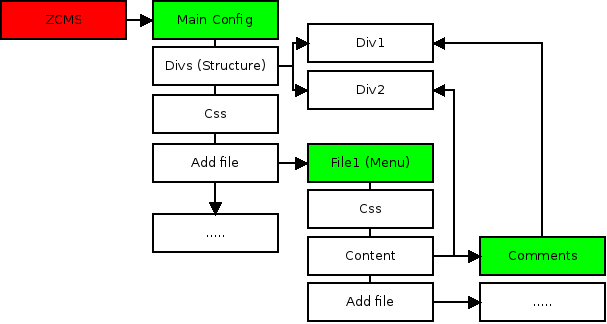
\includegraphics[scale=0.7]{Diagramma_neilos.png} 
\subsection{Menu links}
A typical menu link points to index.html\#!page.xml\ \ .Neilos will load automatically page.xml and will add it to the site with ajax. The file must be located in resources/content/.\\
If the file is not found and no extension is provided, Neilos will try to add .xml and .php extensions to the file name.
\section{Entries Anatomy}
Every file is loaded with an $entryid$ parameter. Neilos search for the entry with the id supplied. For php files, the entry must be enclosed in at least one other element. For xml files, the entry can be the ancestor of the document.\\
An entry consists of 3 main sections: config, title and content. There can be also subentries.\\
Content and title should consist of pure html, since they will be dumped to the DOM.\\
\footnotesize
\begin{minted}{xml}
<entry id='entryid'>
  <config>
    ...
  </config>
  <title>
    ...
  </title>
  <content>
    ...
  </content>


  <!-- Subentries -->
  <entry id='..'></entry>
  <entry id='..'></entry>
</entry>
\end{minted}
\normalsize
\subsection{DOM}
By default, every entry is added to the DOM with a main div ($\#id\_entry$) and 3 subdivs: .title, .content and .comments.\\
This behaviour can eventually be changed with some options (see below). If both $<title>$ and $<content>$ do not exist, the entry is not added to the DOM.
\subsection{Config}
The config tag is useful to load additionals xml,css,php files or to set useful settings.\\
Almost all options are inheritable to subentries. Available options are:
\begin{list}{-}{}
\item \begin{minted}{xml}
<title>       
      \end{minted}
Change the title of the page
\item \begin{minted}{xml}
<css id='css_id'>       
      \end{minted}
Load an external css file. The id is used to identify the css in order to remove or replace it afterwards.
\item \begin{minted}{xml}
<author>m3l7</author>
<date>2011-09-08</date>
      \end{minted}
Specify the date and author of the entry. They will be added to the DOM in the .title before everything else.
\item \begin{minted}{xml}
<structure_div>div_name</structure_div>       
      \end{minted}
Add a div to the DOM. (See Structure section)
\item \begin{minted}{xml}
<target>target</target>       
      \end{minted}
specify where the entry should be added in the DOM (jquery selector).
\item \begin{minted}{xml}
<animation speed='fast' speedshow='normal' speedhide='slow'
 type='fade/slide/hide'>enabled</animation>
      \end{minted}
Select the type and speed of the animation. If speedshow/speedhide is set, it will be used instead of speed for showing/hiding the entry.
The speed can have the format $\#n$, where n is the animation time in milliseconds.
\item \begin{minted}{xml}
<home>#home.xml</home>
      \end{minted}
Set the default home page. See links section for informations about links meaning.
\item \begin{minted}{xml}
<display entries="showfirst/show/hide"></display>
\end{minted}
Choose if content (and comments) should be visible or not. If showfirst is set, the entry is visible only if it's the first child.\\
Default: show
\item \begin{minted}{xml}
<load_file mode='loadwhenshown' 
entryid="menu">resources/xml/menu.xml</load_file>
      \end{minted}
Load an external file. Neilos will add the content inside the jquery selector tag.\\
If mode='loadwhenshown' is set, the file is loaded only when the entry is toggled.
\item \begin{minted}{xml}
<clear>false</clear>
\end{minted}
If true, the target will be cleared before adding the entry. Not inheritable.
\item \begin{minted}{xml}
<skipcontent>true</skipcontent>
\end{minted}
If true, title and content will be ignored.
\item \begin{minted}{xml}
<skipsubentries>true</skipsubentries>
\end{minted}
If true, subentries will be ignored.
\item \begin{minted}{xml}
<type>notitle</type>
\end{minted}
If set, title will be ignored.
\item \begin{minted}{xml}
<default_extension>xml</default_extension>
\end{minted}
Set the default extension of content files. Can be xml or php and can be set only in the main config (config.xml)\\
Neilos will cycle throigh the other extensions automatically if the file is not found.
\item \begin{minted}{xml}
<class>optionalclass</class>
\end{minted}
Add an additional class to the entry.
\item \begin{minted}{xml}
<click prevent_default='true' href='filename' remove='true'></click>
\end{minted}
Open an internal link (specified by href) when the entry is clicked. If prevent\_default is set, the normal toggle behaviour is avoided.\\
If remove is set, the entry is removed after being clicked.
\end{list}
\normalsize
\section{Variables}
Neilos has an internal parser which substitutes some special strings. At this stage, it's very limited.
\begin{list}{-}{}
\item \begin{minted}{javascript}
_$version
\end{minted}
show Neilos version
\end{list}
\normalsize
\section{Structure}
Structure objects can be created using the following methods:
\subsection{js methods}
\begin{list}{-}{}
 \item Neilos.Structure.new\_div: this will create a simple div. Additional classes can be added.
\item Neilos.Structure.new\_tab: this will create an entry (\bfseries{TODO} \normalfont Rename to new\_entry?). An entry is a div with 2 or 3 subdivs: [title], content, comments. Each subdivs has 2 subdivs: \_text and \_text\_right
\end{list}
\subsection{xml methods}
\begin{list}{-}{}
  \item \begin{minted}{xml}
<structure_div>         
        \end{minted}
create a div and a subdiv \_content. It is created at the end of the current DOM, so it should be used only in the main config. It must be placed inside $<$config$>$ tag.
\end{list}

\section{SEO}
Starting from version 1.2.2, Neilos can be indicized by Google, using the standard \_escaped\_fragment method.\\
A load.php and a modified index.php is provided, which can load the site using php only code.
At the moment, load.php loads all the content, but generally not in the correct order and with the correct containers; for this readon it is not suitable for every day use as a replacement for the default js code.

\section{Plugins}
Starting from Neilos 1.3, it is possible to add server side (php) plugins. To use them, one should use as content a simple php file which includes the plugins engine (content\_loader.php), and calls load\_file, which finally loads the real data file (xml or php).\\
The arrays \$plugin[] and \$param[] are used to specify the list of plugins to load and their parameters.\\
Below is reported an example content file


\begin{minted}{php}
<?php
include_once '../plugin/content_loader.php';

$file = 'home.xml';	#real data file
$tag_in='home';		#tag of the data file
$tag_out='home_more';	#tag of the output file

$plugins = array('more');	#list of plugins to load

$param = array();		#parameter array

$param['_more_id']='home';	#id, used to identify univocally this file
$param['_more_home_num_per_page']=3;	#parameters of the more plugin
$param['_more_home_show_more']=1;	#correct syntax is _plugin_id_parameter

load_file($file,$tag_in,$tag_out);
?>
\end{minted}
\subsection{List of plugins}
\subsubsection{more} more\\
more plugin prevents neilos to load the whole content file if the number of entries is big.\\
It is possible to specify how many entries have to be shown at the same time.\\
\bfseries Parameters:\\
\normalfont \normalsize -num\_per\_page: number of entries to display in a single 'page'.\\
-show\_more: if set to 1, a button which loads the next page will be visible.\\
\end{document}